\documentclass[12pt]{article}%
\usepackage{blindtext}
\usepackage{enumitem}
\usepackage{natbib}
\usepackage{graphicx}
\usepackage[table,xcdraw]{xcolor}
\usepackage{geometry}
\usepackage{tabularx}
\graphicspath{{images/}}

\begin{document}

\title{Team Plan}
\date{\today}
\maketitle
\section{Team information}




\begin{itemize}
\item Malin Jakobsen (xun007) - Team leader and documentation maintainer. \\
Responsibility: Maintain house rules and general management of team. Coding, documentation maintenance. \\
	Experience: Has taken part in project management activities before. Has technical
experience through INF100, INF101, INF102.

\item Olav Gjerde (ogj005) - Git repo leader and main game lead. \\
Responsibility: Maintaining the git repo structure, and assisting the other teammates
with the use of git and its features. Is leader of the main game, have overview over code structure. \\
Experience: Has technical expertise through INF100, INF101 and INF102.
\item Keerthan Kumaranayagam (kku007) -  Coder and documentation\\
Responsibility: Presentation and retroperspective updater\\
Experience: INF100, INF101, INF102 and basics within Photoshop.
\item Ole Kristian Solheim Gjerløw (ogj003) - GUI lead\\
Responsibility: Lead of the GUI implementation\\
Experience: INF100, INF101, INF102. Experience with Illustrator/Photoshop if we want to makeour own assets/textures. Some experience with JavaFX.
\item Renate Nikolajeva (rni006) - Documentation\\
Responsibility: Presentation and class diagram\\
	Experience: Had INF100, INF101, INF102. Has some experience in Photoshop and
Vegas Pro.

\item Rune Vatne  (rva013) - Coder and documentation\\
Responsibility:  Demo video maker and sequence diagram creator \\
	Experience: INF100, INF101, INF102.
\item Simen Gad Hasvi  (qax007) - AI lead\\
Responsibility: Class diagram, project structure and lead of the AI implementation.\\
	Experience: Had INF100, INF101 and INF102. No experience with GUI.
  \item Henrik Borgli (hbo019) - Sound and picture manager\\
  Responsibility: Lead on music, sound and other visual logos.\\
  	Experience: Had INF100, INF101 and INF102. JavaFx and other specialities.
\end{itemize}

Roles might change from one iteration to another


\section{House rules}


\begin{itemize}
\item Every individual implementation is “best effort”, meaning that if an individual encounters major problems or notices that they have stagnated they are requested to seek help with the others in the group at the earliest convenience.
\item Meeting with the group at least once per week outside of the obligatory lab is the goal, adding additional meetings may be considered when enough work has been accumulated.
\item Most communication will take place through “Discord”, there will be dedicated channels to programming, tools, guides, documentation and non-project related activities.
\item All code submitted to the repository shall be commented and be properly formatted for easy understanding within the team.
\item If features that are being implemented changes the product in such a way that the documentation needs altering, then this should be written down and notified to the rest of the team.
\end{itemize}


\section{Team repository structure}

\textit{We will use the git-flow “idea” of a git workflow to structure our repository. This means that instead of just working at the master branch, we will have additional branches such as develop, feature, release and in special cases hotfix. Though we may omit some of these at certains parts of the project if it causes to much confusion for the participants.}
\vspace{5mm} %5mm vertical space

The master branch will store the release history of the project, and the develop 		branch will serve as an integration branch which we will be able to merge finished 	feature branches into. Each major feature should have its own branch which then can be pushed to the remote repository for further collaboration. The feature branches are branched off of the latest develop branch.
\vspace{5mm} %5mm vertical space
    Release branches are forked off of the develop branch after the develop branch has acquired enough features. This will be the “product” that will be shipped when the deadline date hits. Only bug fixes, additional documentation and such may be added to the release branch after is has been established. When it is ready the release branch will be merged into the master branch, representing a new version of the product.
Hotfix branches are used for fixing urgent issues with the released product in the master branch, this means that it is forked off of the master branch. When a given fix is complete this should be merged in master and develop.

\vspace{5mm}
\begin{center}
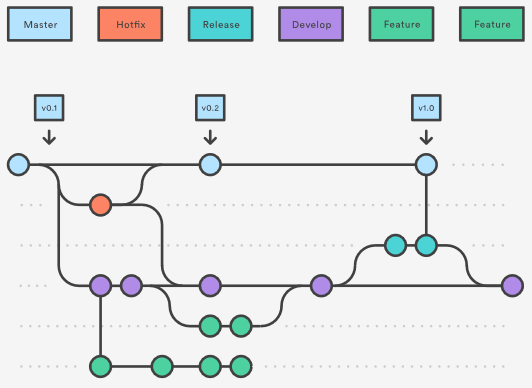
\includegraphics[scale=0.8]{image12.png}\\
\textit{Branch-figure from: (Atlassian, 2018)}
\end{center}
\vspace{5mm}

\noindent
"1. A develop branch is created from master \\
2. A release branch is created from develop \\
3. Feature branches are created from develop \\
4. When a feature is complete it is merged into the develop branch \\
5. When the release branch is done it is merged into develop and master \\
6. If an issue in master is detected a hotfix branch is created from master \\
7. Once the hotfix is complete it is merged to both develop and master" \\
\textit{(Atlassian, 2018)} \\

\noindent
Additionally the folder structure will look something like this: \\ \\
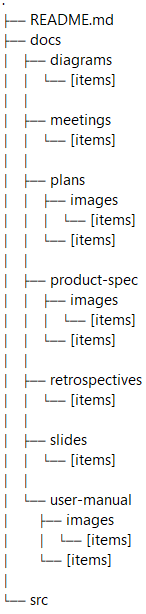
\includegraphics[scale=0.7]{structure.png}
\vspace{5mm}

\vspace{5mm} %5mm vertical space
Initial documentation will be produced with google docs for fast collaboration before being translated into latex and pdf formats. After this changes to the documentation happens through the git repository.



\section{General risk analysis}
This is a list containing the risks that we found most pressing for this project. The list is subject to change, and may also grow as the project progresses.


\begin{tabularx}{\linewidth}{ r X X }
\hline
Risk & Description and Probability & Strategy \\ \hline

Staff Illness
& If staff falls ill in a critical period of development, and is unable to contribute (- Moderate)
& Get an overview of what the individual was working on, if critical, we assign the task to other team members, if not, put on hold.\\

Requirements changes
&If additional requirements are delivered to the team that requires altering of the product (- Moderate)
& Assess the impact the changes will have on the current state of the product and generate a list of the most pressing issues. Allocate workforce by looking at the list.\\ \hline
Underestimated development time
&If the team underestimated the work a feature requires in regards to the deadline (- High)
& Cut back on features that does contribute directly to the main specification of the product, and reallocate team members to the feature features in question.                 \\ \hline
\end{tabularx}

\vspace{30mm}
\section{References}
\begin{itemize}
\item Atlassian (2018) Gitflow Workflow [Internet] \\
	  Available from: \textit{https://www.atlassian.com/git/tutorials/comparing-workflows/
	  gitflow-workflow} \\
	  Read: 20.february 2018\\
	  License: https://creativecommons.org/licenses/by/2.5/au/
\end{itemize}



\end{document}
